% Figure 1 — the heat path and the three ways to cover the hottest hours.
% Final width 174 mm; fonts 7/8/9 pt; relative positioning only.
\documentclass[border=1mm]{standalone}
\usepackage[T1]{fontenc}
\usepackage{helvet}
\usepackage{textcomp}
\renewcommand{\familydefault}{\sfdefault}
\usepackage{tikz}
\usetikzlibrary{positioning,calc,arrows.meta,backgrounds,fit}
\definecolor{mainline}{HTML}{0072B2}
\definecolor{mainfill}{HTML}{E8F3FA}
\definecolor{waterline}{HTML}{9C6500}
\definecolor{waterfill}{HTML}{FFF1CC}
\definecolor{compline}{HTML}{7B3294}
\definecolor{compfill}{HTML}{F1E5F3}
\definecolor{ink}{HTML}{333333}
\definecolor{rule}{HTML}{9E9E9E}
\newcommand{\sev}{\fontsize{7}{8.2}\selectfont}
\newcommand{\eig}{\fontsize{8}{9.4}\selectfont}
\newcommand{\nin}{\fontsize{9}{10.6}\selectfont}
\newcommand{\dC}{\,\textdegree C}
\begin{document}
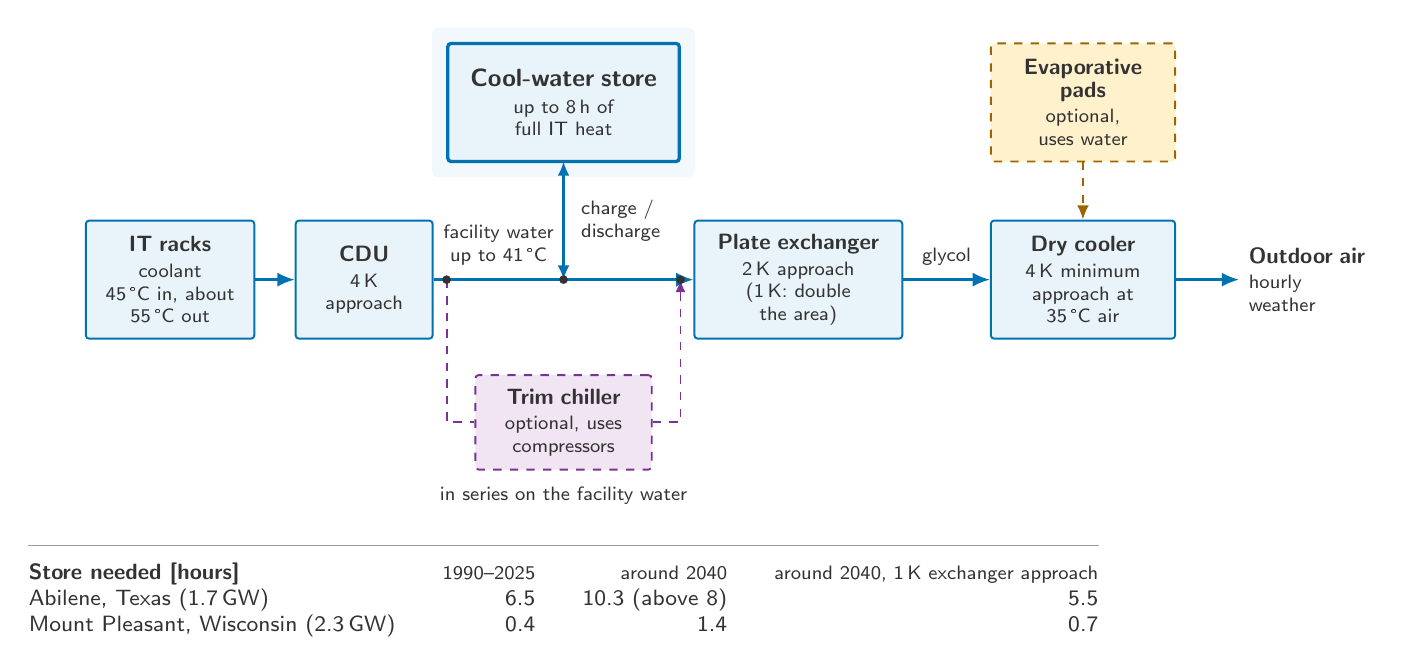
\begin{tikzpicture}[
  font=\sev, text=ink, execute at begin node={\hyphenpenalty=10000\exhyphenpenalty=10000},
  box/.style={draw=mainline, fill=mainfill, line width=0.7pt, rounded corners=1.2pt, align=center,
              minimum height=15mm, inner sep=1.2mm},
  water/.style={box, draw=waterline, fill=waterfill, dashed},
  comp/.style={box, draw=compline, fill=compfill, dashed},
  spine/.style={draw=mainline, line width=0.9pt, -{Latex[length=2.2mm,width=1.8mm]}},
  pipe/.style={draw=compline, line width=0.7pt, dashed},
]
% ---- main spine (row 2)
\node[box, text width=19mm] (racks) {{\eig\bfseries IT racks}\\[0.4mm]coolant\\45\dC{} in, about\\55\dC{} out};
\node[box, text width=15mm, right=5mm of racks] (cdu) {{\eig\bfseries CDU}\\[0.4mm]4\,K\\approach};
\node[box, text width=24mm, right=33mm of cdu] (hx) {{\eig\bfseries Plate exchanger}\\[0.4mm]2\,K approach\\(1\,K: double the area)};
\node[box, text width=21mm, right=11mm of hx] (dc) {{\eig\bfseries Dry cooler}\\[0.4mm]4\,K minimum\\approach at\\35\dC{} air};
\node[right=8mm of dc, align=left, text width=15mm] (air) {{\eig\bfseries Outdoor air}\\[0.4mm]hourly\\weather};
% ---- junction on the facility-water line and its taps
\coordinate (j) at ($(cdu.east)!0.5!(hx.west)$);
\coordinate (tapL) at ($(cdu.east)!0.05!(hx.west)$);
\coordinate (tapR) at ($(cdu.east)!0.95!(hx.west)$);
% ---- store (row 1), pads (row 1), chiller (row 3); the two row-1 boxes share one base line and one height
\coordinate (row1) at ($(j)+(0,15mm)$);
\node[box, line width=1.2pt, text width=27mm, minimum height=15mm, outer sep=0pt, anchor=south] (store) at (j |- row1) {{\nin\bfseries Cool-water store}\\[0.5mm]up to 8\,h of\\full IT heat};
\node[water, text width=21mm, minimum height=15mm, outer sep=0pt, anchor=south] (pads) at (dc |- row1) {{\eig\bfseries Evaporative pads}\\[0.3mm]optional, uses water};
\node[comp, text width=20mm, minimum height=12mm, below=12mm of j] (chiller) {{\eig\bfseries Trim chiller}\\[0.3mm]optional, uses\\compressors};
\node[below=0.8mm of chiller] (series) {in series on the facility water};
% ---- background emphasis on the store only
\begin{scope}[on background layer]
  \node[fit=(store), inner sep=2mm, fill=mainfill!55, draw=none, rounded corners=2pt] {};
\end{scope}
% ---- connections (8)
\draw[spine] (racks) -- (cdu);
\draw[spine] (cdu.east) -- (hx.west);
\draw[spine] (hx) -- (dc);
\draw[spine] (dc) -- (air);
\draw[draw=mainline, line width=0.8pt, {Latex[length=1.8mm,width=1.5mm]}-{Latex[length=1.8mm,width=1.5mm]}] (j) -- (store.south);
\draw[draw=waterline, line width=0.8pt, dashed, -{Latex[length=1.8mm,width=1.5mm]}] (pads) -- (dc);
\draw[pipe] (tapL) |- (chiller.west);
\draw[pipe, -{Latex[length=1.6mm,width=1.3mm]}] (chiller.east) -| (tapR);
\fill[ink] (tapL) circle (0.55mm) (tapR) circle (0.55mm) (j) circle (0.55mm);
% ---- connection labels
\node[above=0.6mm of $(cdu.east)!0.5!(j)$, align=center] {facility water\\up to 41\dC};
\node[right=1mm of $(j)!0.5!(store.south)$, align=left] {charge /\\discharge};
\node[above=0.6mm of $(hx.east)!0.5!(dc.west)$] {glycol};
% ---- running-example strip
\node[below=6mm of series.south, anchor=north, inner sep=0pt] (strip) {%
  \renewcommand{\arraystretch}{1.15}%
  \begin{tabular}{@{}l@{\hspace{6mm}}r@{\hspace{6mm}}r@{\hspace{6mm}}r@{}}
    \eig\bfseries Store needed [hours] & \sev 1990--2025 & \sev around 2040 & \sev around 2040, 1\,K exchanger approach\\
    \eig Abilene, Texas (1.7\,GW) & \eig 6.5 & \eig 10.3 (above 8) & \eig 5.5\\
    \eig Mount Pleasant, Wisconsin (2.3\,GW) & \eig 0.4 & \eig 1.4 & \eig 0.7\\
  \end{tabular}};
\draw[draw=rule, line width=0.4pt] ($(strip.north west)+(0,2mm)$) -- ($(strip.north east)+(0,2mm)$);
\end{tikzpicture}
\end{document}
